\label{ch:small-time}

% In this chapter we have established the existence of an approximate,
% analytic solution for small values of $t$ whose applicability is
% well defined in terms of error rates at the boundaries (BCs) and the
% locations of the images (ICs).
Chapter \ref{ch:galerkin} introduced a semidiscrete (finite element)
Galerkin method for solving the standardized diffusion problem
(\ref{eq:qqq}). The Galerkin method is most appropriate for large
times, since numerical errors are attenuated with increasing diffusion
time $\tilde{t}$. The obvious limitation of the finite element solver
is that there are problems with $(\sigma_{\tilde{y}}, \tilde{t})$ too
small to be resolved with a reasonable finite number of basis
elements. We will call such parameter combinations as belonging to the
\textit{incomputable region} of the solver. For parameters in the
incomputable region, a sufficient condition to flag them as such is if
the numerical derivative of the finite element solution with respect
to the boundary parameters produces a negative value. However, this is
not a \textit{necessary} condition, and in practice this is an
insidious problem: parameter combinations which should be attributed
with a very small likelihoods may be given values orders of magnitude
higher than they should and thus falsely bias any inferential
procedure. Procedures sensitive to such silent numerical
instabilities, such as particle filters, are especially at risk. In
this chapter, we develop a solution applicable in precisely the cases
where the finite element solver fails: small values for
$\tilde{t}$. In addition to having its own well-defined criteria for
appropriate use (namely an upper bound on $\tilde{t}$ as well as an
upper bound on $\tilde{\sigma}$), the analytic form of the
small-$\tilde{t}$ solution provides a way to bound from above the
incomputable region for the finite element solver.


\section{A small-time solution, revisited}
As part of the overall Galerkin method, Chapter \ref{ch:galerkin} in
introduced a small-time approximation for the normalized diffusion
problem \eqref{eq:qqq} via the method of images (see Section
\ref{sec:pde-small-t}). By reflecting the fundamental solution
(i.e. the solution to the governing PDE without the BCs) about the
closest boundary and picking a sufficiently small
$\tilde{t}_\epsilon$, this approximation satisfies the initial
condition and enforces the boundary conditions. However, because the
analytic dependence of this small-time approximation on the boundaries
is only through the location parameters of the reflected image,
differentiating with respect to all four boundaries yields a uniform
zero value in computing the associated density.

\subsection{Uniqueness and Symmetry Condition}
The insufficiency of the previous small-time solution suggests
extending it by performing more than a single reflection about the
boundaries in the construction of the system of images. If there
exists at least one image whose location is the result of at least one
reflection about each of the four boundaries, then it is guaranteed to
have a non-trivial contribution to the density
$\frac{\partial^4}{\partial a_x \partial b_x \partial a_y \partial
  b_y} p(\tilde{x}, \tilde{y}, \tilde{t})$. An immediate problem of
the extension, however, is the uniqueness of the resultant approximate
density function.

To illustrate the problem, consider again the normalized diffusion
problem where $\rho=0$. The fundamental solution to the problem is an
uncorrelated bivariate Gaussian with variances $\tilde{t}$ and
$\tilde{t}\sigma_{\tilde{y}}^2$ in the $\tilde{x}$ and $\tilde{y}$
directions, respectively. The problem setup and a contour plot of the
fundamental solution is shown in Figure
(\ref{fig:normalized-problem-rho-0}). We can construct two systems of
images by carrying out the series of reflections
\begin{align*}
  & \left\{ 1,2,3,4 \right\}, & \left\{ 2,1,3,4 \right\}, &
\end{align*}
which are shown in Figures () and (). Both resultant solutions satisfy
the PDE as well as the IC/BVs for a sufficiently small
$\tilde{t}_\epsilon$. Although not unique, both solutions to the PDE
problem have minimal relative differences, and they both depart from
the true analytic solution minimally. From a numerical implementation
standpoint, there is only near machine-$\varepsilon$ difference
between them. However, the two solutions have a single image whose
location is a function of all four boundaries, and this single image
entirely defines the corresponding density function. Because the
location parameters are different, the density functions of the two
PDE solutions are consequently very different as well over
$\Omega_2$. Assuring uniqueness using the method of images is achieved
by performing an infinite number of reflections, which is not always
possible (see Section \ref{sec:proof} below).

A condition weaker than uniqueness which nonetheless restricts the
solution space is the inherent symmetry of the problem. A sufficient
symmetry condition arises when
$(\tilde{x}_0, \tilde{y}_0) = (0.5, 0.5)$. Reflecting about the
$\tilde{x}-$ and $\tilde{y}-$axes centered on $0.5$ preserves the
governing PDE, as well as the IC/BVs. Under this transformation, any
realized path of the original diffusion process has the same
likelihood as its transformed version evaluated under the diffusion
measure. In order for the sum of images solution to obey this symmetry
condition, the proposed system of images must be preserved under this
transformation. Further, if we require that the system of images
contain the fewest possible elements, then the unique system is the
union of the sets of reflections
\begin{align*}
  \left\{ 1,2,3,4 \right\} \cup \left\{ 2,1,3,4 \right\} \cup \left\{ 1,2,4,3 \right\} \cup \left\{ 2,1,4,3 \right\}.
\end{align*}
When $(\tilde{x}_0, \tilde{y}_0) = (1/2,1/2)$, the symmetry condition
maps reflections to each other and the set of images is closed
\begin{align*}
  \{1,2,3,4 \} & \to \{2,1,4,3 \}, \\
  \{2,1,3,4 \} &\to \{1,2,4,3 \}, \\
  \{1,2,4,3 \} &\to \{2,1,3,4 \}, \\
  \{2,1,4,3 \} &\to \{1,2,3,4 \}.
\end{align*}

% As in Chapter 2, we can scale,
% rotate, and scale again the problem, so that the boundaries of the
% computational domain have changed, but the fundamental solution to the
% problem is defined by an uncorrelated bivariate Gaussian distribution
% with variance $t$ in each direction. The transformed problem is shown
% in Figure (\ref{fig:transformed-problem-rho-0}).
% The topology under the transformed problem (under $T_{(3)}$ in
% \eqref{eq:T3}) permits the repeated reflection of the fundamental
% solution about the boundaries without any of the images falling within
% the computational domain $\Omega_3$. This further allows for
% subsequent images for fall further from the domain (scaling linearly
% in distance) so that there exists an asymptotic series composed of an
% infinite number of reflections which enforce the IC/BCs and satisfy
% the governing PDE. 

\begin{figure}
  \centering
  %%
  %%
  \begin{tabular}{cc}
    \begin{minipage}{0.40\textwidth}
      \centering
      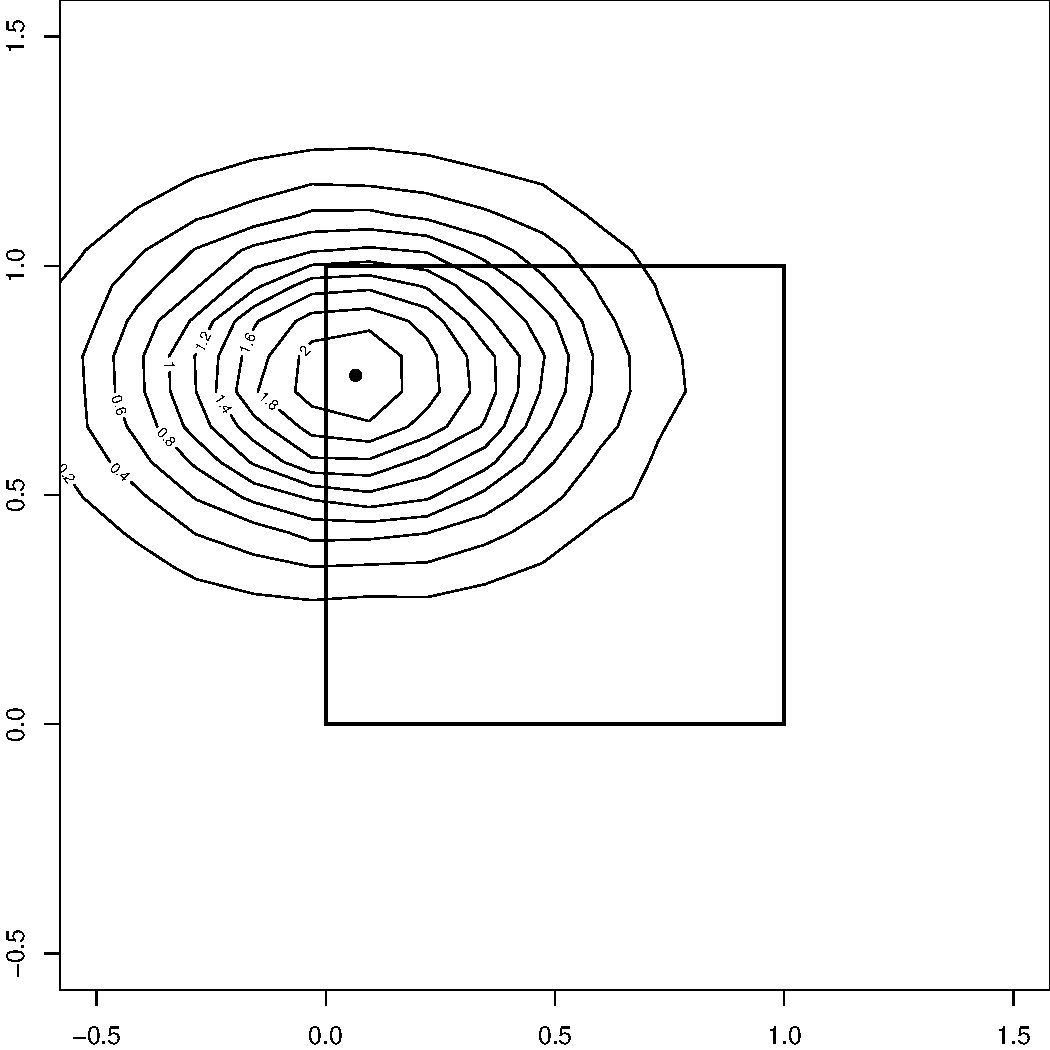
\includegraphics[width=1\linewidth]{../chapter-3/illustration-rho-0-normalized.pdf}
      \caption{The computational domain $\Omega_2$ for the normalized
        problem (\ref{eq:qqq}) is the unit square centered on
        $(0.5,0.5)$. Level sets of the fundamental solution
        with $\rho = 0$ and $\sigma_{\tilde{y}} < 1$ are also shown at an
        initial condition in the upper-left corner of $\Omega_2$.}
      \label{fig:normalized-problem-rho-0}
    \end{minipage}
    %%
    & \begin{minipage}{0.40\textwidth}
      \centering
      \includegraphics[width=1\linewidth]{illustration-rho-0-transformed.pdf}
      \caption{The problem in Figure
        (\ref{fig:normalized-problem-rho-0}) is scaled by
        $1/\tilde{\sigma}$ in the $y-$direction, then rotated $\pi/4$
        counter-clockwise, then scaled again in the principal axes
        direction in order to eliminate the mixing term in the
        resultant PDE problem. Since $\rho=0$ here, the final scaling
        is the identity transformation and the boundaries remain
        orthogonal. The fundamental solution is symmetric under
        rotations centered on the IC under the new topology, as shown
        here.}
      \label{fig:transformed-problem-rho-0}
    \end{minipage}
  \end{tabular}
\end{figure}

We can compose such a finite system of images by reflecting about each
of the boundaries a number of times and picking the greatest possible
time $t^{*}$ such that all boundaries are either numerically or
analytically enforced. One candidate for such a set of reflections is
shown in Figure (\ref{fig:illustration-1}), where the set of images is
produced by the reflections (left, right, left, top, bottom, top). The
solid colored points are image positions having non-zero derivatives
with respect to all four boundary parameters. The green points bound a
symmetric solution respect to a family of transformations centered the
IC (red).
\begin{figure}
  \begin{tabular}{cc}
    \begin{minipage}{0.40\textwidth}
      \centering
      \includegraphics[width=1\linewidth]{../chapter-3/chapter-3-figure-illustration-1.pdf}
      \caption{A finite system of images resultant from the sequence
        of reflections (left, right, left, top, bottom, top), where
        ``left'' refers to left boundary of $\Omega$ running along
        $x=0$, ``right'' refers to the right boundary along $x=1$,
        etc. The red point is the initial condition
        $(x_0,y_0) = (0.1, 0.3)$ which centers the fundamental
        solution. All points outside $\Omega$ are image position
        resulting from the reflections, where the solid colored points
        have positions dependent on $(x_0,y_0)$ \textit{as well as all
          of the boundaries.} The green colored points are symmetric
        about the IC with respect to horizontal and vertical
        reflections centered on $(x_0, y_0)$. The blue points are also
        dependent on all four boundaries, but they violate such
        transformations centered on $(x_0, y_0)$.}
      \label{fig:illustration-1}
    \end{minipage}
    %%
    & \begin{minipage}{0.40\textwidth}
      \centering
      \includegraphics[width=1\linewidth]{chapter-3-figure-illustration-rel-error.pdf}
      \caption{Relative error across $\Omega$ on a $30 \times 30$
        regular grid based on solution (\ref{eq:small-time-sol}) for
        the symmetric distribution of images in Figure
        (\ref{fig:illustration-1}). The max admissible small time
        $t^*$ is bounded above by $0.058$ and used here. The relative
        error rate is on the order of $0.01\%$}
      \label{fig:illustration-rel-error}
    \end{minipage}
      \end{tabular}
\end{figure}
The resultant approximate \textit{small-time solution} to the PDE is
the finite sum of the above images:
\begin{equation}
  \bar{q}(x, y, t^{*}|\tilde{\sigma}) = \sum_{j=1}^J \mbox{sign}_j
  G(x,y|t^*, \tilde{\sigma}, \rho, x_0^{(j)}(a_x, b_x, a_y, b_y, \rho, \tilde{\sigma}),
  y_0^{(j)}(a_x, b_x, a_y, b_y, \rho, \tilde{\sigma})), \label{eq:small-time-sol}
\end{equation}
where $G(\cdot)$ is a bivariate Gaussian density with location
parameters $(x^{(j)}_0,y^{(j)}_0)$ dependent on a set of reflections indexed by $j$ and a
covariance matrix independent of $j$ and determined by
$(\tilde{\sigma}, t^*, \rho = 0)$:
\[
  t^{*} \left( \begin{array}{cc}
                 1 & \rho\tilde{\sigma} \\
                 \rho\tilde{\sigma} & \tilde{\sigma}^2
               \end{array} \right).
\]
The parameters $(a_x,b_x,a_y,b_y)$ define $\Omega$ and are identically
$a_x =0, b_x=1, a_y=0,b_y=1$ for the normalized problem here. We can
control the relative error of the approximation by setting the minimum
absolute value of $\bar{q}$ at the boundaries and solving for
$t^{*}$. For a boundary error rate of at most $1 \cdot 10^{-12}$, the
solution based on the distribution bound by the symmetric (green)
images from Figure (\ref{fig:illustration-1}) produces palatable
relative errors across $\Omega$ compared to the true closed-form
solution, as shown in Figure (\ref{fig:illustration-rel-error}) where
the maximum relative error on a $30 \times 30$ grid is $O(10^{-5})$.
Decreasing the error rate on the boundary to $1 \cdot 10^{-14}$ forces
$t^* \approx 0.047$ and the max relative error on the same grid is
$O(10^{-6})$.

Out of the $J=36$ images in the system considered, nine have location
parameters that are dependent on all four boundary parameters (green
and blue points in Figure (\ref{fig:illustration-1})). Differentiating
$\bar{q}$ with respect to all of the boundary parameters produces an
approximate small-time solution for the full problem that is dependent
upon that subset of the images:
\begin{align}
  \frac{\partial^4 \bar{q}(x, y, t^{*})}{\partial a_x
  \partial b_x \partial a_y \partial b_y} &= \sum_{j^*=1}^{J^*} \frac{\partial^4
                                            G(x,y|t^{*}, \tilde{\sigma}, \rho, x_0^{(j^*)}(a_x, b_x, a_y, b_y, \rho, \tilde{\sigma}),
                                            y_0^{(j^*)}(a_x, b_x, a_y, b_y, \rho, \tilde{\sigma}))} {\partial a_x \partial b_x
                                            \partial a_y \partial b_y}. \label{eq:analytic-solution-rho-0}
\end{align}
One approach to compute the derivatives in
(\ref{eq:analytic-solution-rho-0}) is to numerically perturb the
boundary parameters $(a_x,b_x,a_y,b_y)$ and use a finite difference
approximation directly on the sum
(\ref{eq:analytic-solution-rho-0}). However, since the small-time
solution generally requires the use of a small time $t^* << 1$,
numerical underflow makes direct application of finite difference
hopeless.

We can, however, leverage the very tractable analytic form of the
Gaussian kernel $G(\cdot)$. Given
\begin{align}
  & G(x,y | t^{*}, \tilde{\sigma}, \rho, x_0^{(j^*)}(a_x, b_x, a_y, b_y, \rho, \tilde{\sigma}),
    y_0^{(j^*)}(a_x, b_x, a_y, b_y, \rho, \tilde{\sigma})) = &  \nonumber \\
  & \frac{1}{2\pi\,\, t^{*}\tilde{\sigma}\sqrt{1-\rho^2}} \exp\left( -\frac{1}{2\,\,t^*\, \tilde{\sigma}^2 (1-\rho^2)} \left[ \left(x-x_0^{(j)}\right)^2 \tilde{\sigma}^2 + \left(y-y_0^{(j)}\right)^2 - 2\rho(x-x_0^{(j)})(y-y_0^{(j)})\tilde{\sigma} \right]\right), & \label{eq:full-form-G}
\end{align}
we can define the following factors to more easily express the
higher-order derivatives applied to (\ref{eq:full-form-G})
\begin{align}
  \mathcal{C}(t^*, \tilde{\sigma}, \rho) &:= -\frac{1}{2\,\,t^*\, \tilde{\sigma}^2 (1-\rho^2)}, \\
  \mathcal{P}_j(x,y | \tilde{\sigma}, \rho, a_x,b_x,a_y,b_y) &:= \left(x-x_0^{(j)}\right)^2 \tilde{\sigma}^2 + \left(y-y_0^{(j)}\right)^2 - 2\rho(x-x_0^{(j)})(y-y_0^{(j)})\tilde{\sigma}.
\end{align}
The two key observations here are that $\mathcal{P}(\cdot)$ is
independent of $t^{*}$, meaning $\mathcal{C}(\cdot)$ carries the
$t^{*}$ dependency in differentiation and that only $\mathcal{P}$ is
dependent on the boundary parameters. Without loss of generality,
beginning with $\partial/\partial a_x$ we compute all derivatives:
\begin{align}
  \frac{\partial}{\partial a_x} G(x,y|t^{*}, \tilde{\sigma}, \rho, x_0^{(j^*)}, y_0^{(j^*)}) &= G \cdot \mathcal{C}\,\,\cdot \left( \frac{\partial \mathcal{P}}{\partial a_x} \right)\\
  \frac{\partial^2}{\partial a_x \partial b_x} G(x,y|t^{*}, \tilde{\sigma}, \rho, x_0^{(j^*)}, y_0^{(j^*)}) &= G \cdot \mathcal{C}^2 \left( \frac{\partial \mathcal{P}}{\partial b_x} \right) \left( \frac{\partial \mathcal{P}}{\partial a_x} \right) + G \cdot \mathcal{C} \cdot \left( \frac{\partial^2 \mathcal{P}}{\partial a_x \partial b_x} \right) \\
  %% %% %%
  \frac{\partial^3}{\partial a_x \partial b_x \partial a_y} G(x,y|t^{*}, \tilde{\sigma}, \rho, x_0^{(j^*)}, y_0^{(j^*)}) &= G \cdot \mathcal{C}^3 \left( \frac{\partial \mathcal{P}}{\partial b_x} \right) \left( \frac{\partial \mathcal{P}}{\partial a_x} \right) \left( \frac{\partial \mathcal{P}}{\partial a_y} \right) \nonumber \\
                                                                                             &\,\, + G \cdot \mathcal{C}^2 \left[\left( \frac{\partial^2 \mathcal{P}}{\partial a_x \partial a_y} \right) \left( \frac{\partial \mathcal{P}}{\partial b_x} \right) + \left( \frac{\partial^2 \mathcal{P}}{\partial b_x \partial a_y} \right) \left( \frac{\partial \mathcal{P}}{\partial a_x} \right) + \left( \frac{\partial^2 \mathcal{P}}{\partial a_x \partial b_x} \right) \left( \frac{\partial \mathcal{P}}{\partial a_y} \right)\right] \nonumber \\
                                                                                             &\,\, + G \cdot \mathcal{C} \left( \frac{\partial^3 \mathcal{P}}{\partial a_x \partial b_x \partial a_y} \right) \nonumber \\
                                                                                             %% %% %%
  \frac{\partial^4}{\partial a_x \partial b_x \partial a_y \partial b_y} G(x,y|t^{*}, \tilde{\sigma}, \rho, x_0^{(j^*)}, y_0^{(j^*)}) &= G \cdot \mathcal{C}^4 \cdot \left(\partial_{a_x}\partial_{b_x} \partial_{a_y}\partial_{b_y} \right)\mathcal{P} \nonumber \\
                                                                                             &\,\, + G \cdot \mathcal{C}^3 \cdot \left( \partial^2_{a_x\, b_x} \partial_{a_y} \partial_{b_y} + \partial^2_{a_x\, a_y} \partial_{b_x} \partial_{b_y} + \partial^2_{a_x\, b_y} \partial_{b_x} \partial_{a_y} + \right. \nonumber \\
                                                                                             & \left. \qquad\qquad\qquad +\partial^2_{b_x\, a_y} \partial_{a_x} \partial_{b_y} + \partial^2_{b_x\, b_y} \partial_{a_x} \partial_{a_y} \partial^2_{a_y\, b_y} \partial_{a_x} \partial_{b_x} \right) \mathcal{P} \nonumber \\
                                                                                             &\,\, + G \cdot \mathcal{C}^2 \cdot \left( \partial^3_{a_x\,b_x\,a_y} \partial_{b_y} + \partial^2_{a_x\,b_x}\partial^2_{a_y\,b_y} + \partial^3_{a_x\,b_x\,b_y}\partial_{a_y}  + \right. \nonumber \\
                                                                                             & \left. \qquad\qquad\qquad + \partial^3_{a_x\,a_y\,b_y} \partial_{b_x} + \partial^2_{a_x\,a_y} \partial^2_{b_y\,b_x} + \partial^3_{b_x\,a_y\,b_y}\partial_{a_x} + \partial^2_{b_x\,a_y}\partial_{a_x}\partial_{b_y} \right) \mathcal{P} \nonumber \\
                                                                                             &\,\, + G \cdot \mathcal{C} \cdot \partial^4_{a_x\,b_x\,a_y\,b_y} P. \label{eq:fourth-deriv}
\end{align}
With (\ref{eq:fourth-deriv}), we can express each of the derivatives
in (\ref{eq:analytic-solution-rho-0}) as the sum of derivatives of the
polynomial $\mathcal{P}$ with respect to the boundary parameters. In
particular, derivatives in (\ref{eq:fourth-deriv}) avoid the previous
numerical underflow problems and lend themselves to finite difference
approximation even at high orders.

Thinking of $t^{*}$ as variable allows us to further simplify
(\ref{eq:fourth-deriv}). Since $\mathcal{C} = \mathcal{O}(1/t^{*})$,
all three terms $G\cdot \mathcal{C}^3, G\cdot \mathcal{C}^2,$ and
$G\cdot \mathcal{C}$ are
$o\left( G\cdot \mathcal{C}^4 \cdot \left(\partial_{a_x}\partial_{b_x}
    \partial_{a_y}\partial_{b_y} \right)\mathcal{P} \right)$, so that
the $G\cdot \mathcal{C}^4$ order term in (\ref{eq:fourth-deriv})
dominates the others for sufficiently small $\,\,t$. This truncation,
when appropriate, is useful for reducing computational complexity
\textit{and} it guarantees that the numerical implementation of the
derivatives produces positive values for all $t$ as long as
$\left(\partial_{a_x}\partial_{b_x} \partial_{a_y}\partial_{b_y}
\right)\mathcal{P}$ is positive. Truncating at $\mathcal{C}^4$, the
analytic likelihood approximation given by the sum of images is of the
form:
\begin{align}
  &\frac{\partial^4 \bar{q}(x, y, t)}{\partial a_x
  \partial b_x \partial a_y \partial b_y} \approx  & \nonumber \\
  &\sum_{j} \left\{ \frac{1}{2\pi\,\, t\tilde{\sigma}\sqrt{1-\rho^2}} \exp\left(
    -\frac{1}{2\,\,t^*\, \tilde{\sigma}^2 (1-\rho^2)} \left[
      \left(x-x_0^{(j)}\right)^2 \tilde{\sigma}^2 +
      \left(y-y_0^{(j)}\right)^2 -
      2\rho(x-x_0^{(j)})(y-y_0^{(j)})\tilde{\sigma} \right]\right)
    \cdot \right. & \nonumber \\
  &\qquad \qquad \left. \left( -\frac{1}{2\,\,t^*\, \tilde{\sigma}^2 (1-\rho^2)} \right)^4 \cdot \left(\partial_{a_x}\partial_{b_x}
    \partial_{a_y}\partial_{b_y} \right)\mathcal{P} \right\}. & \label{eq:truncated-approx}
  % & \propto IG\left( t^* | \alpha = 4, \beta = -\frac{1}{2\, \tilde{\sigma}^2 (1-\rho^2)} \left[
  %     \left(x-x_0^{(j)}\right)^2 \tilde{\sigma}^2 +
  %     \left(y-y_0^{(j)}\right)^2 -
  %     2\rho(x-x_0^{(j)})(y-y_0^{(j)})\tilde{\sigma} \right] \right)
\end{align}
The above approximate solution is close to the true existing
small-time solution for $t < t^*$. Extending beyond $t^*$ produces a
positive function dominated by the exponential term $G$. Figure
(\ref{fig:illustration-likelihood-profile}) shows a profile comparison
of the log-likelihood with respect to $t$ for the example
configuration used so far. The truncated approximate solution tracks
well with the true solution up to $\mathcal{O}(t) = 1$. Closer
observation of (\ref{eq:truncated-approx}) reveal that each of the
summands are proportional to an Inverse-Gamma distribution, since
$\left(\partial_{a_x}\partial_{b_x} \partial_{a_y}\partial_{b_y}
\right)\mathcal{P}$ is not dependent on $t$. This allows us to
approximate the value for $t$ which maximizes the likelihood function
(see Section (\ref{sec:modes}) below).
\begin{figure}
  \begin{tabular}{c}
    \begin{minipage}{0.90\textwidth}
      \centering
      \includegraphics[width=1\linewidth]{chapter-3-figure-illustration-likelihood-profile.pdf}
      \caption{Log-likelihood profile comparison between small-time
        truncated solution (as given in (\ref{eq:truncated-approx}),
        solid black line) and the true analytic solution (red
        points). The small time for which the approximation is valid
        is $\log(t^*) \approx -9$. We see that in this example the
        truncated approximation deteriorates for $\mathcal{O}(t) = 1$,
        well after the technical bound set by $t^*$.}
      \label{fig:illustration-likelihood-profile}
    \end{minipage}
  \end{tabular}
\end{figure}
Applying a first-order finite difference approximation with a finite
step $\Delta = 10^{-5}$ to compute the polynomial derivatives produces
relative errors with a maximum of order $\mathcal{O}(10^{-4})$ on the
same $30 \times 30$ grid used for Figure
(\ref{fig:illustration-rel-error}), as shown in Figure
(\ref{fig:illustration-rel-error-likelihood}).
\begin{figure}
  \centering
  \begin{tabular}{c}
    \begin{minipage}{0.50\textwidth}
      \centering
      \includegraphics[width=1\linewidth]{chapter-3-figure-illustration-rel-error-likelihood.pdf}
      \caption{Relative error for the likelihood problem comparing the
        true solution with the truncated small-time approximation in
        (\ref{eq:truncated-approx}) on a $30 \times 30$ regular grid
        over $\Omega$. }
      \label{fig:illustration-rel-error-likelihood}
    \end{minipage}
    \end{tabular}
    % %%
    % & \begin{minipage}{0.40\textwidth}
    %   \centering
    %   \includegraphics[width=1\linewidth]{chapter-3-figure-illustration-rel-error-likelihood.pdf}
    %   \caption{}
    %   \label{fig:illustration-rel-error-likelihood-truncated}
    % \end{minipage}
    %   \end{tabular}
\end{figure}

% \begin{figure}
%   \centering
%   %%
%   %%
%   \includegraphics[scale=0.8]{illustration-rho-0-all-configurations.pdf}
%   \caption{All 24 non-unique systems of images that result from
%     reflecting about each of the boundaries once. Blue dots represent
%     location parameters of images whose weight is positive, while
%     green dots represent locations of images with negative
%     weights. The red dot is the image location that is a function of
%     all four boundaries.}
%   \label{fig:all-configurations}
% \end{figure}


\subsection{Counterexample with $\rho \neq 0$}
For $\rho=0$, the above procedure is guaranteed to produce an
admissible set of images regardless of the IC configuration and
$\tilde{\sigma}$ used. However, this is not the case for a general
combination of $\rho$ and $\tilde{\sigma}$. Consider Figure
(\ref{fig:counterexample-1}), which features the same configuration of
parameters and reflections as above, except that $\rho=0.9$. We can
see that applying the above procedure produces a system with images
within the computational domain, violating the IC.  However, below we
prove that for any IC and $\rho$ combination, we can find a
sufficiently small $\tilde{\sigma}$ such that a series of reflections
used in the illustration will yield a valid system of images.
\begin{figure}
  \begin{tabular}{cc}
    \begin{minipage}{0.50\textwidth}
      \centering
      \includegraphics[width=1\linewidth]{chapter-3-figure-counterexample-1.pdf}
      \caption{When $\rho=0.9$, the system of images generated by the
        set of reflections in Figure (\ref{fig:illustration-1}) now
        violates the IC as at least one of the images falls within
        $\Omega$. }
      \label{fig:counterexample-1}
    \end{minipage} &
    %%
    \begin{minipage}{0.50\textwidth}
      \centering
      \includegraphics[width=1\linewidth]{chapter-3-figure-proof-1.pdf}
      \caption{Geometry characteristic of the transformed problem when
        $\rho>0$. The thick dashed line defines the axis along which
        images resultant from reflecting about boundaries 2 and 4
        fall. The blue point denotes the intersection of the axis and
        the extension of boundary 3.}
      \label{fig:proof-1}
    \end{minipage} \\
    %%
    \begin{minipage}{0.50\textwidth}
      \centering
      \includegraphics[width=1\linewidth]{chapter-3-figure-proof-3.pdf}
      \caption{Set of images in the original topology when
        $\tilde{\sigma} = 0.1$. All images fall outside of $\Omega$
        for $\rho = 0.9$.}
      \label{fig:proof-3}
    \end{minipage} &
        \begin{minipage}{0.50\textwidth}
      \centering
      \includegraphics[width=1\linewidth]{chapter-3-figure-proof-2.pdf}
      \caption{Set of images in the transformed topology when
        $\tilde{\sigma} = 0.1$. All images fall outside of $\Omega$
        for $\rho = 0.9$.}
      \label{fig:proof-2}
    \end{minipage}
  \end{tabular}
\end{figure}

\section{Existence of valid systems of images} \label{sec:proof}
\begin{lemma}
  Given $\rho > 0$, and $(x_0, y_0) \in \Omega$, there
  exists $0 < \tilde{\sigma} \leq 1$ such that
  $(x_0^{(j)}, y_0^{(j)}) \notin \Omega, \forall \, j\in
  \left\{1, \ldots, J\right\}$, where the collection of image
  locations $\left\{1, \ldots, J\right\}$ is the result of a finite
  set of reflections about the boundaries of $\Omega$.
\end{lemma}

\begin{proof}
  Given that in the standard problem $\Omega$ is a unit square
  whose lower-left corner is centered on the origin, applying the
  transformation $T$ produces a characteristic geometry for the IC/BV
  problem that is illustrated in Figure (\ref{fig:proof-1}). Corners
  a) and c) are obtuse, while b) and d) are acute. Further, lines
  $(1,3)$ and $(2, 4)$ are each parallel and of the same length, with
  lines 2 and 4 being longer. This can be observed from the
  coordinates of the four corners defining $\Omega$ in the transformed
  topology:
  \begin{align*}
    a &= (0,\quad 0),&
                       b &= \frac{\sqrt{2}}{2} \left( \frac{1}{\sqrt{1-\rho}},\quad \frac{1}{\sqrt{1+\rho}} \right), \\
    c &= \frac{\sqrt{2}}{2} \left( \frac{1-1/\tilde{\sigma}}{\sqrt{1-\rho}},\quad \frac{1+1/\tilde{\sigma}}{\sqrt{1+\rho}} \right),&
                                                                                                                                     d &= \frac{\sqrt{2}}{2} \left( \frac{-1/\tilde{\sigma}}{\sqrt{1-\rho}},\quad \frac{1/\tilde{\sigma}}{\sqrt{1+\rho}} \right), \\
    IC &= \frac{\sqrt{2}}{2} \left( \frac{x_0 - y_0/\tilde{\sigma}}{\sqrt{1-\rho}},\quad \frac{x_0 + y_0/\tilde{\sigma}}{\sqrt{1-\rho}} \right)
  \end{align*}

  Now consider placing the images $j = 1, \ldots, J$ by performing a
  finite number of alternating reflections about lines 4 and 2. This
  places images along a finite segment of a line running through the
  IC position and orthogonal to lines 2 and 4 (dashed line and
  black/red dots in Figure (\ref{fig:proof-1})). If the number of
  reflections is kept constant, $\tilde{\sigma}$ can be sufficiently
  small such that all thus placed images are in the interior region
  formed by extending lines 1 and 3. This is proved from the following
  observations:
  \begin{enumerate}
  \item The slopes of both lines 2 and 4 are equal to
    $-\frac{\sqrt{1+\rho}}{\sqrt{1-\rho}}$ and are therefore
    \textit{independent of the choice} of $\tilde{\sigma}$. Hence,
    shrinking $\tilde{\sigma}$ moves corners d) and c) along lines 4
    and 2, respectively, away from the origin and thereby increasing
    the interior region formed by extending lines 1 and 3.
  \item From observation i), the length of the chord covering the
    reflection line within $\Omega$ is a constant independent of
    $\tilde{\sigma}$.  This implies that the length of the finite
    segment covering the reflected images is also constant and
    independent of $\tilde{\sigma}$.
  \item The coordinate of the point of intersection between the
    reflection line and the extension of line 3 (blue point in Figure
    (\ref{fig:proof-1})) is
    \[
      \frac{\sqrt{2}}{2} \left( \frac{-2 x_0\rho + 2
          y_0/\tilde{\sigma} -
          2/\tilde{\sigma}(1-\rho)}{-2\rho\sqrt{1-\rho}},
        \frac{\sqrt{1-\rho}}{\sqrt{1+\rho}}\frac{-2 x_0\rho + 2
          y_0/\tilde{\sigma} -
          2/\tilde{\sigma}(1-\rho)}{-2\rho\sqrt{1-\rho}} +
        \frac{1}{\sqrt{2}\tilde{\sigma}\sqrt{1+\rho}} \right).
    \]
    The lengths of the $x-$ and $y-$segments of the chord connecting
    the IC and the point of intersection are
    \begin{align*}
      \Delta x &= \frac{\sqrt{2}}{2}\left\{ \frac{1}{\tilde{\sigma}}\cdot\frac{\tilde{\sigma}x_0 - y_0/\rho + (1-\rho)/\rho + y_0}{\sqrt{1-\rho}} - \frac{x_0}{\sqrt{1-\rho}} \right\},\\
      \Delta y &= \frac{\sqrt{2}}{2} \left\{ \frac{1}{\tilde{\sigma}}\cdot\frac{(\tilde{\sigma}x_0 - 2y_0/\rho + (1-\rho)/\rho + 1/\sqrt{2})\sqrt{1-\rho} - y_0\sqrt{1+\rho}}{\sqrt{1-\rho}\sqrt{1+\rho}}- \frac{x_0}{\sqrt{1-\rho}} \right\}.
    \end{align*}
    Hence, as $\tilde{\sigma} \to 0$, both $\Delta x^2 \to \infty$ and
    $\Delta y^2 \to \infty$, so that the distance between the point of
    intersection and the IC grows. The symmetry of the problem (in
    terms of reflections $x \to -x$ and $y \to -y$) makes the argument
    applied to line 3 and the line of reflection applicable to the
    extension of line 1 as well. Figures (\ref{fig:proof-2}) and
    (\ref{fig:proof-3}) show the reflected images falling within the
    interior region with $\tilde{\sigma} = 0.1$ in both geometries.
  \end{enumerate}
  Observations ii) and iii) imply that we can always find a
  sufficiently small $\tilde{\sigma}$ to cover the line segment
  containing the positions of images resulting from a finite number of
  reflections about boundaries 2 and 4.  Hence, any subsequent
  reflections about lines 1 and 3 are guaranteed to place reflected
  images outside of the computational region $\Omega$.

  For any such finite, admissible collection of images, we can make
  $t^*$ sufficiently small such that the BVs are numerically
  enforced on three out of the four boundaries (since with a finite
  set of reflections the BVs are analytically enforced at the last
  boundary of reflection). Therefore, we have a collection of images
  $J$ whose sum satisfies the IC/BV problem \textit{and} is
  nontrivially differentiable with respect to the four boundary
  parameters for $\Omega$.
\end{proof}

\section{Lack of Uniqueness and Symmetry Condition}
From the above Lemma and the illustration so far, it is obvious that
the finite set of images satisfying the IC/BV problem is not unique. 


Retaining the minimum number of images necessary to satisfy the
symmetry condition forces us retain the four images defined by the
reflections $\{1,2,3,4 \},\{2,1,3,4 \},\{1,2,4,3 \},\{2,1,4,3 \}$ and
thereby define our small-time solution. The previous Lemma guarantees
the existence of such a set of images satisfying the IC/BV problem for
a sufficiently small $\tilde{\sigma}.$ 


\section{Approximate Solution over $t$} \label{sec:modes}
% In this chapter we have established the existence of an approximate,
% analytic solution for small values of $t$ whose applicability is
% well defined in terms of error rates at the boundaries (BCs) and the
% locations of the images (ICs).
Chapter 2 introduced a semi-analytic (Galerkin) finite element method
for solving the standardized diffusion problem
(\ref{eq:standard-diffusion}). Unlike the small-time solution, the
Galerkin method is most appropriate for ``large'' times, since it
attenuates numerical errors with increasing $t$. The obvious
limitation of the finite element solver is that there are problems
with $(\tilde{\sigma}, t)$ too small to be resolved with a reasonable
finite number of basis elements. We will call such parameter
combinations as belonging to the \textit{incomputable region} of the
solver. For parameters in the incomputable region, a sufficient
condition to flag them as such is if the numerical derivative of the
finite element solution with respect to the boundary parameters
produces a negative value. However, this is not a \textit{necessary}
condition, and in practice this is an insidious problem: parameter
combinations which should be attributed with a very small likelihoods
may be given values orders of magnitude higher than they should and
thus falsely bias any inferential procedure. Procedures sensitive to
such silent numerical instabilities, such as particle filters, are
especially at risk.

On the other hand, the approximate solution developed in this chapter
is applicable in precisely the cases where the finite element solver
fails: small values for $t$. In addition to having its own
well-defined criteria for appropriate use (namely an upper bound on
$t$ as well as an upper bound on $\tilde{\sigma}$ that produces images
outside of $\Omega$), the analytic form of (\ref{eq:truncated-approx})
provides a way to bound from above the incomputable region for the
finite element solver. As mentioned earlier, each of the summands in
(\ref{eq:truncated-approx}) are proportional to an Inverse-gamma
distribution with the parameters
\begin{align*}
  \alpha_j &= 4,& \beta_j &= -\frac{1}{2\, \tilde{\sigma}^2 (1-\rho^2)} \left[
                        \left(x-x_0^{(j)}\right)^2 \tilde{\sigma}^2 +
                        \left(y-y_0^{(j)}\right)^2 -
                        2\rho(x-x_0^{(j)})(y-y_0^{(j)})\tilde{\sigma} \right]
\end{align*}
The mode of each of the summands is, therefore,
$\beta_j/(\alpha_j+1)$. The summand with the smallest $\beta_j$
contributes the most to the truncated small-time solution, so that the
smallest mode $\beta_j/(\alpha_j+1)$ is closest to the mode of
the approximating function. Even though the truncated solution is not
applicable for all $t$, its mode still gives a reasonable
approximation for the $t$ value which maximizes the true likelihood
function. An empirical validation is discussed below (see Figures
(\ref{fig:modes-histogram}) - (\ref{fig:modes-scatterplot})), which
provide views of the errors in approximating the true
value $t$ maximizing the likelihood and the approximation derived from
the truncated small-time solution:
\[
  \min_{j} \{ \beta_j/(\alpha_j+1) \} - t_{\max},
\]
where $t_{\max}$ is the $t$ value maximizing the true likelihood (for
$\rho=0$) given some parameter combination $(x_0, y_0, x_t, y_t)$ and
$\tilde{\sigma}$. Each data point in the histogram/scatterplot
corresponding to such a combination was generated by sampling
\begin{align*}
  \sigma_x &\sim \mbox{Lognormal}(2, 2), & \sigma_y &\sim \mbox{Lognormal}(2, 2), & \rho &= 0,
\end{align*}
then simulating from a bivariate Brownian motion using a forward Euler
method and a small time step. Normalizing to the standard diffusion
problem (see equation (\ref{eq:standard-diffusion})), $t_{\max}$ was
found numerically conditional on $(x_0, y_0, x_t, y_t)$ and
$\tilde{\sigma}$, since we have the closed-form likelihood for the
$\rho=0$ case. For the same input parameters, we generate four images
as given by our method above and then find
$\min_{j} \{ \beta_j/(\alpha_j+1) \}$. We compare how the
Galerkin solution performs at this boundary of the computable region
and beyond in the figures below.

The histogram in Figure (\ref{fig:modes-histogram}) shows the
distribution of signs and magnitudes of the error differences in
approximating the modes
$t_{\mbox{max}} - \min_{j} \{ \beta_j/(\alpha_j+1) \}$, which are
correlated with small $\tilde{\sigma}$ (Figure
(\ref{fig:modes-scatterplot})). Further, can see from the plot of true
mode vs. error in Figure (\ref{fig:modes-scatterplot-2}) that largest
errors occur for modes that are large on relative to the
$t-$scale. The distribution of true log-likelihood values at the
approximate modes is given in Figure (\ref{fig:modes-histogram-2}). We
can see that these function values are relatively large and should be
resolvable by the finite element solver. This is finally confirmed in
Figure (\ref{fig:modes-histogram-3}), which shows the relative error
using the FE solver.
\begin{figure}
  \begin{tabular}{cc}
    \begin{minipage}{0.50\textwidth}
      \centering
      \includegraphics[width=1\linewidth]{chapter-3-figure-validation-modes-histogram.pdf}
      \caption{A histogram of differences
        $t_{\max} - \min_{j} \{ \beta_j/(\alpha_j+1) \}$ between the
        approximate mode of the truncated small-time solution and the
        true mode of closed-form solution, when $\rho=0$. We see that
        the order magnitude of error in approximating the true point of
        maximum for the likelihood function is 0.1, where the bias is
        towards underestimating the mode.}
      \label{fig:modes-histogram}
    \end{minipage} &
    \begin{minipage}{0.50\textwidth}
      \centering
      \includegraphics[width=1\linewidth]{chapter-3-figure-validation-modes-scatterplot.pdf}
      \caption{Scatterplot of $\tilde{\sigma}$ vs.
        $\min_{j} \{ \beta_j/(\alpha_j+1) \} -
        t_{\max}$. Larger approximation errors in the
        mode point are correlated with smaller
        $\tilde{\sigma}$.}
      \label{fig:modes-scatterplot}
    \end{minipage}  \\
    \begin{minipage}{0.50\textwidth}
      \centering
      \includegraphics[width=1\linewidth]{chapter-3-figure-validation-modes-scatterplot-2.pdf}
      \caption{Scatterplot of true mode value vs.
        $\min_{j} \{ \beta_j/(\alpha_j+1) \} - t_{\max}$. Larger
        approximation errors in the mode point are correlated with
        higher mode locations.}
      \label{fig:modes-scatterplot-2}
    \end{minipage} &
    \begin{minipage}{0.50\textwidth}
      \centering
      \includegraphics[width=1\linewidth]{chapter-3-figure-validation-modes-histogram-2.pdf}
      \caption{Histogram of log-likelihood values at approximate mode
        locations.  We can see that, with respect to machine
        $\epsilon$ the true function values at the approximate modes
        are large and ought to be resolved by the finite element
        solver.}
      \label{fig:modes-histogram-2}
    \end{minipage}
  \end{tabular}
\end{figure}

\begin{figure}
  \begin{tabular}{c}
    \begin{minipage}{0.90\textwidth}
      \centering
      \includegraphics[width=1\linewidth]{chapter-3-figure-validation-modes-histogram-3.pdf}
      \caption{Histogram of relative error of FEM solver at the
        approximate modes.}
      \label{fig:modes-histogram-3}
    \end{minipage}
  \end{tabular}
\end{figure}